\documentclass[12 pt]{book}
\usepackage{amsmath}
\usepackage{amsthm}
\usepackage[paperwidth=5 in,paperheight=5 in,left=7 mm, right=7 mm, top=15 mm, bottom=16 mm]{geometry}
\usepackage{graphics}
\usepackage{fontawesome}
\usepackage{enumitem}
\usepackage{marvosym}
\newcommand{\myitem}{\refstepcounter{enumi}\item[$^\star$\theenumi.]}
\newcommand{\mmyitem}{\refstepcounter{enumi}\item[$^{\star \star}$\theenumi.]}
\setcounter{page}{01}

\usepackage[utf8]{inputenc}
\usepackage{xcolor}
\setlength{\arrayrulewidth}{0.1 mm}
%BLUE%
%\definecolor{Mycolor2}{HTML}{3D9BE9}
\definecolor{Mycolor2}{HTML}{33cccc}
%\definecolor{Mycolor2}{HTML}{000000}

%%----HEADER &&& FOOTER----%%

\usepackage{fancyhdr}


\pagestyle{fancy}
\fancyhf{}
\setlength{\headheight}{8 mm}
%\fancyhead[CE,CO]{ \Times\Large{\textbf{\textls*[100]{\textcolor{tomato}{\textit{Illustration}}}}}}

\fancyhead[CE,CO]{\Large{\textbf{\textls*[250]{\textcolor{tomato}{SOLVE ME! \\[-5 mm]{\Large{\textbf{\textls*[5000]{\textcolor{black}{\scalebox{.42}{ROTATION}}}}}}     }}}}}

%\fancyfoot[CE,CO]{\Large{\textls*[10]{\textcolor{tomato}{\Times\textit{\tikz \draw [-{Stealth[red]}, line width=4.5,line cap=round] (0,0) node[below=-13.5 mm,scale=2.2,below left]{\textbf{Solution}}--(1.65,0);}}}}}

\renewcommand{\headrulewidth}{0 mm}
\renewcommand{\footrulewidth}{0 mm}


\DeclareMathOperator{\Ln}{ln}

%%----FONT &&& MATHS_FONT----%%

\usepackage{amssymb}
\usepackage{upgreek,xspace}
\newcommand*{\rom}[1]{\expandafter\@\romannumeral #1}


\usepackage[utopia]{mathdesign}
\renewcommand{\familydefault}{\sfdefault}
\usepackage[scaled=1]{helvet}
\newcommand*\Times{\fontfamily{ptm}\selectfont}

%%%------PACAKAGES------%%%

\usepackage[letterspace=120]{microtype}
\usepackage{enumitem}
\usepackage{multicol}
\usepackage{pgfplots}
\pgfplotsset{width=8cm,compat=1.16}
\usepackage{tikz}
\usepgfplotslibrary{fillbetween}
\usetikzlibrary{quotes,angles,patterns,through,calc}
\usepgflibrary{arrows.meta}
\usetikzlibrary{decorations.pathmorphing}
\usetikzlibrary{decorations.markings}
\usetikzlibrary{arrows.meta,bending}
\usepackage{rotating}
\usepackage{tikz-3dplot}
\include{tikz-3dplot}
\usepackage[american voltages, american currents,siunitx]{circuitikz}
\usepackage{circuitikz}
\usetikzlibrary{fit,positioning}
\usetikzlibrary{optics}
\usetikzlibrary{intersections}
\usetikzlibrary{decorations.pathreplacing}
\usepgflibrary{decorations.shapes}
\usepackage{setspace}
\setstretch{1.1}
\usepackage{tkz-tab} [3]
\usepgflibrary{fadings}



\usepackage{vwcol}[widths={0.25,0.75}]


\usepackage{color}
\usepackage[autostyle]{csquotes}


\usepackage{xcolor}
\definecolor{Mycolor2}{HTML}{33cccc}
\definecolor{One}{HTML}{336666}
\definecolor{Two}{HTML}{666666}
\definecolor{Three}{HTML}{cc6699}


%  black--brown--black %
\definecolor{Four}{HTML}{000000}
\definecolor{Five}{HTML}{330000}
\definecolor{Six}{HTML}{000000}

\definecolor{Seven}{HTML}{ff6666}
\definecolor{Eight}{HTML}{330066}
\definecolor{Nine}{HTML}{cc3333}
\definecolor{tomato}{HTML}{FF6347}
\definecolor{darkblue}{HTML}{2c3e50}
\definecolor{blackm}{HTML}{363636}
\definecolor{pink}{HTML}{ff6666}





\tikzset{
bigger/.style={decoration={shape start size=.25cm, shape end size=1cm}}, smaller/.style={decoration={shape start size=1cm, shape end size=.25cm}}, decoration={shape backgrounds,
shape sep={.25cm, between borders},shape scaled}
}



  \tikzset{every to/.style={append after command={[draw,dashed]}}}

\tikzset{
  mirror->/.style={postaction={decorate,black!95,draw,thick,
decoration={border,amplitude=-0.25cm,angle=45,segment length=0.22cm,pre length=0.5 mm}}
  }
}



\def\centerarc[#1]#2(#3)#4(#5:#6:#7)% [draw options] (center) (initial angle:final angle:radius)
  {\draw[#1]($(#3)+({#7*cos(#5)},{#7*sin(#5)})$)arc(#5:#6:#7);}



\newcommand{\sm}{\begin{minipage}[c]{0.1\linewidth}
{\Huge{\textcolor{tomato}{\textbf{ }}}}
\end{minipage}}

\newcommand{\AxisRotator}[1][rotate=0]{%
    \tikz [x=0.25cm,y=0.60cm,line width=.2ex,-stealth,#1] \draw (0,0) arc (-120:120:1 and 1);%
}


%%%%%%       Problem Number        %%%%%%%%
%%%%%%       Problem Number        %%%%%%%%

\newcommand{\nm}{\begin{minipage}[c]{0.1\linewidth}
{\Huge{\textcolor{tomato}{\textbf{18. }}}}
\end{minipage}}

%%%%%%       Problem Number        %%%%%%%%
%%%%%%       Problem Number        %%%%%%%%

\newcommand{\vl}{{{\textcolor{tomato}{\textbf{\vrule width 2.25 pt{}}}}}}

\newenvironment{question}
{	
	\nm  \vl \,
	\begin{minipage}[l]{0.86\linewidth}
	\begin{itshape}
	\normalsize\Times\textit{}
}
{
	\end{itshape}
	\end{minipage}
}


\newenvironment{options}
{	
	\sm ~
	\begin{minipage}[l]{0.86\linewidth}
	\begin{multicols}{2}
	\begin{enumerate}[label={(\roman*)}, itemsep=4 mm]
	\normalsize{}
}
{
	\end{enumerate}
	\end{multicols}
	\end{minipage}
}


\newenvironment{v-options}
{	
	\sm ~
	\begin{minipage}[l]{0.86\linewidth}
	\begin{enumerate}[label={(\roman*)}, itemsep=4 mm]
	\normalsize{}
}
{
	\end{enumerate}
	\end{minipage}
}



\newenvironment{definition}
{
	\begin{center}
	\begin{itshape}
	\normalsize\Times\textit{}
}
{
	\end{itshape}
	\end{center}
}


\newenvironment{note}
{
	\begin{center}
	\begin{itshape}
	\normalsize\Times\textit{}
}
{
	\end{itshape}
	\end{center}
}


\newenvironment{calculations}
{
	\begin{itshape}
	\normalsize\Times\textit{}
}
{
	\end{itshape}
}


\newenvironment{q-options}
{	
	\sm ~
	\begin{minipage}[l]{0.86\linewidth}
	\begin{note}
	\begin{enumerate}[label={(\roman*)}, itemsep=1 mm]
	\normalsize{}
}
{
	\end{enumerate}
	\end{note}
	\end{minipage}
}



\newcommand{\physics}{\normalsize{\textcolor{tomato}{\textls*[100]{{\hspace*{75 mm} @10xphysics}}}}}
\newcommand{\solution}{\centering\Large\Times\textbf{\textcolor{tomato}{\textls*[100]{ \textit{\\[-20 mm]Solution}}} }}
\newcommand{\calculation}{\centering\large\Times{\textcolor{tomato}{ \textit{\\[-18 mm]calculations:\\}} }}
\newcommand{\integration}{\centering\large\Times{\textcolor{tomato}{ \textit{\\[-18 mm]Integration involved:\\[-2 mm]}} }}
\def\step[#1]{\Times{\textcolor{tomato}{\textbf{\textit{Step-#1.}}}}}

\newcommand{\ans}{\Times{\textcolor{red}{ \textit{$\quad$Ans.}}}}


\begin{document}


\nopagecolor
%\boldmath
\color{black!100}
%\pagecolor{black!95}
\setlength{\parindent}{0pt}
\large


\begin{question}
A rotating ball hits a rough horizontal plane with a vertical velocity $v$ and angular velocity $\omega$. Given that the coefficient of friction is $\upmu$ and the vertical component of the velocity after collision is $v/2$, find the angular velocity after the collision.
\end{question}

{\physics}

\begin{center}
\begin{tikzpicture}[>=Stealth,very thick,every node/.style={scale=0.85}, every node/.style={color=red}]
\draw[mirror->] (-3,-1.25)--(3,-1.25);
\draw (0,1.5) edge[->] node[at end,right]{$v$} (0,-0.6) circle[radius=1.5];
\fill [red] (0,1.5) circle(2pt);
\centerarc [->] (0,1.5)(130:-60:0.7);
\node at (0.7,1.5)[right]{$\omega$};
\end{tikzpicture}
\end{center}

\pagebreak


\pagestyle{empty}

\begin{center}
{\solution}
\end{center}


\begin{calculations}
\step[1] This is the case of collision of rigid body therefore during collision normal force acting on the sphere will be impulsive in nature hence it is of much greater magnitude in compare to weight of sphere, so in the equation of linear impulse we can ignore its weight.
\begin{align*}
\textit{Linear Impulse} &= \textit{Change in linear momentum} \\[4 mm]
\int N \; dt&=\Delta p \\[4 mm]
				&= m\Delta v \\[4 mm]
				&=m \left( \dfrac{v}{2} - \left( -v \right)  \right) \\[4 mm]
				&=\dfrac{3mv}{2} \\
\end{align*}

\step[2] Now apply the equation for angular impulse, keep in mind that here the friction force (\textcolor{red}{$f_r=\upmu N$}) acting on the sphere will also be impulsive in nature.
\begin{align*}
\textit{Angular Impulse} &= \textit{Change in angular momentum} \\[4 mm]
\int \tau \; dt&=\Delta L \\[4 mm]
-\;\int  R f_r \; dt &= I \Delta \omega \\
\end{align*}
\tikz \filldraw[black,fill=red,very thick] (0,0) circle (3.5 pt);
Negative sign indicates that torque due to friction is responsible for decreasing the angular velocity hence the angular momentum.
Think in this way :
Initially angular velocity is in clockwise direction means during collision friction will start acting in rightward direction and this friction force will try to rotate the sphere in anti-clockwise direction, in this process angular velocity will start to decrease.
\begin{align*}
- \; \int R \left(\upmu N \right) \; dt &= I \Delta \omega \\[ 3mm]
- \; R \upmu \int N \; dt &= I \left( \omega_f - \omega_i \right) \\[3 mm]
- \; R\upmu \left( \dfrac{3mv}{2} \right) &= \dfrac{2}{5}mR^2 \left( \omega_f - \omega_i \right) \\[3 mm]
\omega_f &= \omega - \dfrac{15\upmu v}{4R} \ans
\end{align*}
\end{calculations}
{\physics}

\pagebreak

\begin{center}

\begin{tikzpicture}[decoration=brace,scale=2]
 %\draw [help lines] grid (3,2); 
 \draw [decorate,very thick] (0,0) -- (0,2);
\end{tikzpicture}
\end{center}


\begin{tikzpicture}
  \draw [help lines] grid (3,2);
  \fill [decorate,bigger,
decoration={shape sep={.25cm, between borders}}, blue!50] (0,1.5) -- (3,1.5);
\fill [decorate,smaller,
decoration={shape sep={1cm, between centers}}, red!50]
(0,.5) -- (3,.5);
\draw [gray, dotted] (0,1.625) -- (3,2) (0,1.375) -- (3,1)
(0,1) -- (3,.625) (0,0) -- (3,.375);
\end{tikzpicture}

\begin{tikzpicture}[>=Stealth]
\draw[put coordinate=A at 0.1,put coordinate=B at 0.9] (0,0) -- (1.5,1) -- (3, 0) -- (4.5,1);
\draw[red] (A) -- (B);
\fill(A) circle (2pt) node[above] {A} ;
\fill(B) circle (2pt) node[above] {B} ;
%\draw [->] (0,0) -- (1.5,-1);
%\draw (0,0)  to[short dim arrow={label'=$l$,no raise,label near middle},red] (2,0);
\draw (0,0)  to[short dim arrow={label=$l$,no raise,label near middle},red] (2,0);
\draw[put coordinate=a at 0.2,put coordinate=b at 0.8,very thick] (0,-2)--(5,-2);
\fill [red] (a) circle(2pt) (b) circle(2pt); 
\end{tikzpicture}


\begin{tikzpicture}[line cap=round,line width=3pt]
\filldraw [fill=yellow!80!black] (0,0) circle (2cm);
  \foreach \angle / \label in
    {0/3, 30/2, 60/1, 90/12, 120/11, 150/10, 180/9,
     210/8, 240/7, 270/6, 300/5, 330/4}
  {
\draw[line width=1pt] (\angle:1.8cm) -- (\angle:2cm);
\draw (\angle:1.4cm) node{\textsf{\label}}; }
\foreach \angle in {0,90,180,270}
\draw[line width=2pt] (\angle:1.7cm) -- (\angle:2cm);
\draw (0,0) -- (120:0.8cm); % hour
\draw (0,0) -- (90:1cm); % minute 
\end{tikzpicture}%



\end{document}